\documentclass[a4paper, 12pt]{article}
%%\usepackage[italian]{babel}
\usepackage[utf8x]{inputenc}
\usepackage{amssymb}
\usepackage{amsthm}
\usepackage{wrapfig}
\usepackage{titlesec}
\usepackage{geometry}
\usepackage{tikz}
\usetikzlibrary{arrows,automata,positioning}
\graphicspath{ {./immagini/} }
\frenchspacing
\newcommand{\subtitle}[1]{%
  \posttitle{%
    \par\end{center}
    \begin{center}\large#1\end{center}
    \vskip0.5em}%
}
\titleformat*{\section}{\Large}
\geometry{a4paper, top=2cm, bottom=2cm, left=2.5cm, right=2.5cm,  heightrounded, bindingoffset=5mm}
\title{Informatica Teorica}
\author{Stefano Staffolani, Filippo Speziali}
\date{ Anno accademico 2022-2023}
\newtheorem{theorem}{Theorem}[section]
\newtheorem{lemma}[theorem]{Lemma}
\newtheorem{corollary}{Corollary}[theorem]
\begin{document}
\maketitle
\tableofcontents
\newpage
\section{Puntate precedenti}
qui metto quello che manca dalle lezioni precedenti....
\section{La macchina di Turing}
Una macchina di Turing \`e una tupla $\langle \sum, Q,q_0,H,\delta\rangle$. Dove: 
\begin{enumerate}
\item $\sum$ \`e un \textbf{alfabeto} di simboli, che include un simbolo speciale $\emptyset$ che indica una cella vuota.
\item $Q$ \`e un insieme finito di \textbf{stati}.
\item $q_0 \in Q$ \`e lo stato iniziale.
\item $H \subset Q$ \`e l'insieme degli \textbf{stati accettanti (o finali)}.
\item $\delta$ \`e la funzione di transizione $\delta: (Q \backslash H) \times \sum \rightarrow Q \times \sum \{ \rightarrow, \leftarrow \} $
\end{enumerate}
$\delta$ esprime il programma che governa il funzionamento della TM, ed \`e una funzione totale. Possimao scrivere la definizione di $\delta$ come un insieme di quintuple.
\subsection{Espressivit\`a delle macchine di Turing}
Molto spesso un problema che vogliamo risolvere usando uno strumento di calcolo pu\`o essere espresso come un problema di decisione. Ad esempio\begin{itemize}
\item Dato un grafo, \`e strettamente connesso?
\item Dato un insieme di equazioni, ha una soluzione?
\end{itemize}
\section{WHILE un linguaggio di programmazione di alto livello	}
Turing-completo: quando il suo potere espressivo e' equivalente ad una macchina di Turing. 
Quindi quando qualcuno scrive un nuovo linguaggio deve preoccuparsi del fatto che esso sia Turing-complete.
Non tutti i linguaggi sono Turning-Completi. Ad esempio i domain specific language.
Sintassi in maniera informale:
\begin{enumerate}
\item 1) assegnazione di variabili X:=3
\item 2) cicli while   while X!=Y do Program
\item 3) sequenziamento di programmi  program1; program2; program3
\item 4) altri costrutti come it-then-else possono essere definiti a partire da questi primitivi.
\end{enumerate}  1) assegnazione di variabili X:=3
NB: NON ci sono side-effects(tipo print(42))
\subsection{Semantica}
Un programma WHILE calcola una funzione paziale da \(N^{K} -> N^{K} \) 
\subsection{Equivalenza}
\begin{theorem}
Una funzione (parziale ) é computabile da un programma WHILE se e solo se é computabile da una macchina di Turing.
\end{theorem}
\begin{proof}
La dimostrazione e` per induzione sulla struttura di un programmma WHILE, supponiamo basato su variabili \(X_1...X_k\)
\begin{enumerate}
\item Caso base
	Se il programma e` un'assegnazione di 0 ad una variabile:
	\(begin X_j := 0 end\) la TM corrispondente e` quella che su input rimpiazza il valore di \(X_j\) con 0.
	Gli altri casi base sono il programma vuoto e le altre due forme di assegnazione.
\item Caso induttivo
	Ci sono due casi da considerare: sequenza e ciclo while.
	\begin{itemize}
	\item sequenza
		per II abbiamo un programma della forma \(begin P_1;P_2;...;P_j end\)
		dove \(P_1,...\) sono programmi per i quali abbiamo, da ipotesi induttiva, TM equivalenti M1,... rispettivamente. La TM per \( begin P_1;...;P_j end\) e` definita nel seguente modo a partire da esse, dove l'output di Mi viene dato come input di Mi+1.
	\item ciclo while
	Assumiamo un programma della forma \(begin while X_{i} != X_j do P end \) dove P e` un programma per il quale, da ipotesi induttiva, abbiamo un aTM M  equivalente. Possiamo costruire una TM \(M_{test}\) che rigetta l'input se il valore di \(X_{i} e X_{j}\) e` diverso, ed accetta altrimenti. La TM per il nostro programma e` costruita come segue: (snapshot da inserire)
	\end{itemize}
\end{enumerate}
\end{proof}

\section{Macchina di Turing Universale}
\subsection{Programmi universali} 
Un programma universale e` un programma pensato per ricevere altri programmi come input ed eseguirli. I sistemi operativi sono esempi di programmi universali.\\
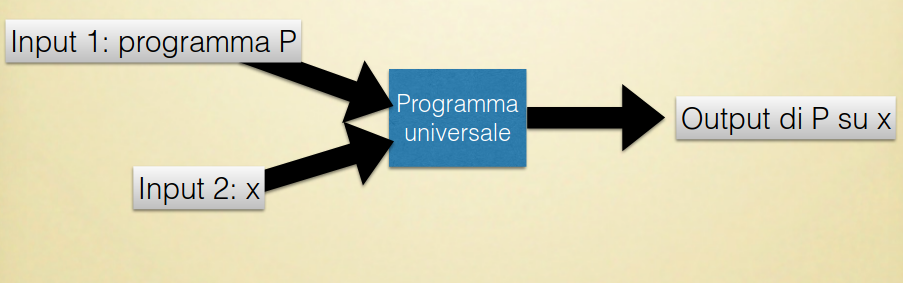
\includegraphics[scale=0.5]{programmi_universali.png}
Anche gli interpreti sono programmi universali.\\
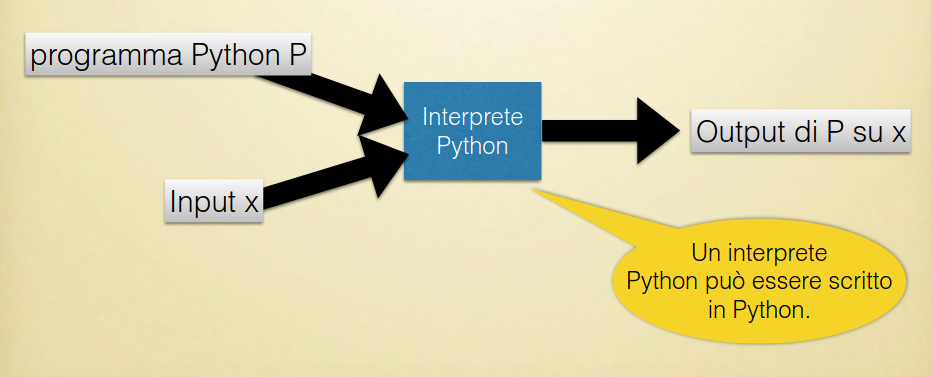
\includegraphics[scale=0.5]{interpreti_programmi_universali.png}
\subsection{La macchina di Turing universale (UTM)}
La UTM prende in input una stringa y, e per prima cosa verifica che y sia della forma code(M)code(x), dove code() e` una codifica, M e` un TM, e x una stringa nell'alfabeto di input \(\sigma_i di M.\)
Se e` cosi`, allora la UTM simula l'esecuzione di M siu x.\\ 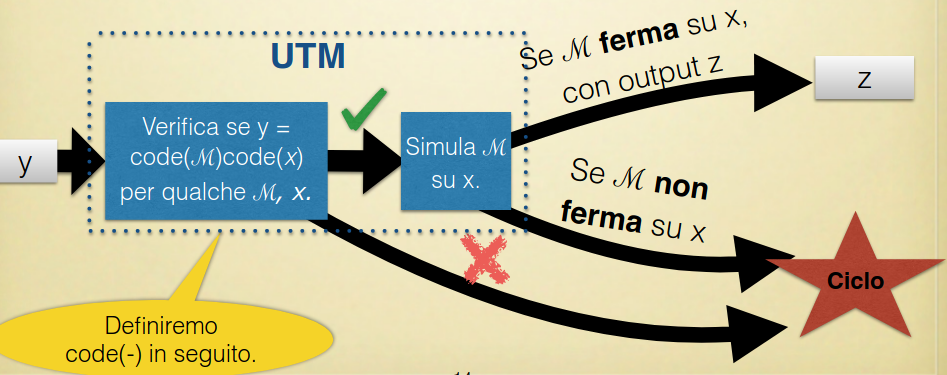
\includegraphics[scale=0.5]{UTM.png}
\subsection{Codificare una TM}
\(M = (\sigma, Q, q_0, H, \delta)\)
Introduciamo alcune convezioni. Gli stati in Q sono ordinati come \(q_0,q_1,...\) con \(q_0\) iniziale. Ordiniamo i simboli che possono apparire nella definizione di \(\delta\)
\[\sigma0 = \emptyset \   \ \sigma1 = \rightarrow \    \ \sigma2=\leftarrow \]
e gli altri simboli in \(\sigma\) come \(\sigma4,..\)
Possiamo codificare gli stati ed i simboli come stringhe unarie: \[code(q_i) = 11...1 \   \ code(\sigma_i)=11...1\]
Codifichiamo una tupla t di $\delta$ come: \[code(t) =code(q_i)0code(\sigma_n)0code(q_j)0code(\sigma_m)0code(\sigma_0)0\]
E la funzione di transizione $\delta={t_1,t_2,...,t_k}$ come \[code(\delta) = code(t_1)0code(t_2)0...0code(t_k)0\]
Possiamo dedurre quali sono gli stati finali di H: sono quelli su cui $\delta$ non e` definita (= non occorrono mai in terza posizione in una tupla).
INSERIRE ESEMPIO
\subsection{Osservazioni sulla codifica}
E` possibile che ci siano due o piu' TM che computino la stessa funzione, ma codificate come stringhe differenti (intuitivamente: se esprimono un diverso algoritmo). Nondimeno, la codifica e` \(iniettiva\): due macchine differenti saranno codificate da stringhe differenti. Data una stringa su {0,1}, e` possibile determinare se sia o meno il codice di una TM (e di quale). In particolare: si tratta di un problema \textbf{decidibile}.\\
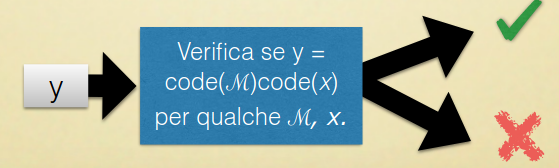
\includegraphics[scale=0.6]{codifica_UTM.png}

\subsection{Costruzione di una UTM}
La UTM e` definita come una macchina di Turing con tre nastri. 
\begin{enumerate}
\item Nastro 1 mantiene il nastro di M in forma codificata.
\item Nastro 2 manterra` code(M).
\item Nastro 3 manterra` o stato corrente di M in forma codificata.
\end{enumerate}
Un passo della simulazione di  M da parte della UTM funziona nel seguente modo.
\begin{enumerate}
\item Cerca in code(M) una tupla $⟨ q_i, \sigma_n, q_j, \sigma_m, \sigma_o ⟩$ dove qi concida con lo stato sul nastro 3 e $\sigma_n$ coincida con il simbolo attualmente esaminato da M.
\item Aggiorna nastro 1 con il nuovo simbolo $\sigma_0$ e sposta la testina nella direzione $\sigma_m$.
\item Aggiorna nastro 3 con lo stato $q_j$. Se é finale, fermati.
\end{enumerate}
\subsection{Considerazioni finali}
Questa costruzione mostra l'esistenza di una macchina di Turing universale, $M_U$. Niente impedisce a $M_U$ di ricevere la sua stessa codifica code($M_U$) come parte dell'input! Questa forma di autoreferenzialita` sara` utilizzata nella prossima lezione per dimostrare che esiste un problema indecidibile.

\section{Cosa non possono fare le TM}
Introduciamo il nostro primo problema indecidibile: il problema della \textbf{fermata}($halting\ problem$). Questo risultato ci informa, pi\`u in generale, sui limiti della computazione per algoritmi. Abbiamo visto che l'essere calcolabile da una procedura algoritmica implica essere calcolabile da una TM. Dunque \textbf{non} essere calcolabile da una TM implica non essere calcolabile da nessuna procedura algoritmica.
\subsection{Ripasso: Linguaggi e TM}
\begin{theorem}
Una TM $M$ \textbf{decide} un linguaggio \textbf{L} se:
\begin{enumerate}
\item Quando $x \in L$, allora $M$ accetta $x$(= ferma nello stato Y).
\item Quando $x \notin L$, allora $M$ rigetta $x$(= ferma nello stato N).
\end{enumerate}
\end{theorem}

\begin{theorem}
Una TM $M$ \textbf{riconosce} un linguaggio \textbf{L} se:
\begin{enumerate}
\item Quando $x \in L$, allora $M$ termina.
\item Quando $x \notin L$, allora $M$ non termina.
\end{enumerate}
\end{theorem}
\subsection{Gradi di (in)calcolabilit\`a}
\begin{enumerate}
\item Decidibile da una TM se e solo se \`e calcolabile($\exists$ un algoritmo che risponde "Si" o "No").
\item Non decidibile da nessuna TM ma riconoscibile da una qualche TM se e solo se non \`e calcolabile(Semi-decidibile: nessun algoritmo sapr\`a calcolare tutte le risposte "No").
\item Non riconoscibile da nessuna TM se e solo se non \`e calcolabile(del tutto non calcolabile: qualsiasi algoritmo fallir\`a nel dare sia le risposte "Si" che "No").
\end{enumerate}
\subsection{Un problema indecidibile: Halting Problem}
Supponiamo che esista un a codifica $code(-)$ che presa una TM su alfabeto $\sum$ restituisce le stringhe $x \in \sum^*$. La codifica usata per definire la macchina di Turing universale \`e un esempio di tale procedura.
Definiamo il linguaggio del \textbf{problema della fermata}:
\begin{center}
HALT = \{(y,x) $\in \sum^*$x$\sum^*|$ y = code($M$) $e$ $M$ ferma su x. \}
\end{center} 
\begin{theorem}
\label{th:1}
Il problema della fermata \`e riconoscibile ma non \`e decidibile.
\end{theorem}
\begin{proof}
Dimostriamo che HALT \`e riconoscibile$^{[1]}$ e che non \`e decidibile$^{[2]}$.\\
\begin{enumerate}
\item Dimostriamo che HALT \`e riconoscibile. Dobbiamo costruire una TMU $M_H$ che prende in input una coppia $(y,x)$, se $y$ ferma su $x$ $M_H$ si ferma altrimenti cicla.
\item dimostriamo che HALT non \`e decidibile. Assumiamo che HALT sia decidibile, e chiamiamo $M_H$ la TM che decide HALT. Perci\`o $M_H$ si comporter\`a come segue. Se $y=code(M)$ per un qualche $M$: \\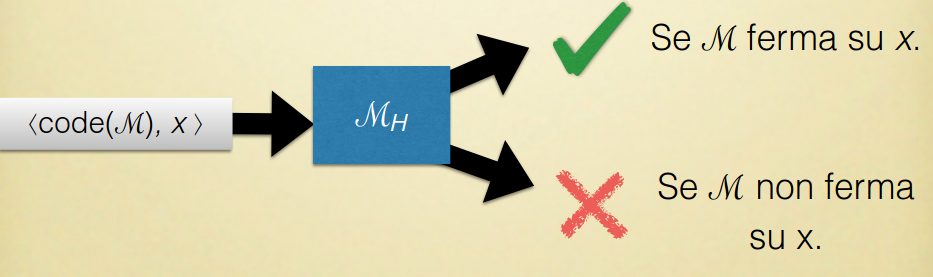
\includegraphics[scale=0.4]{TM_HALT1.png}\\
Possiamo definire una nuova TM $M'$ come segue.\\ 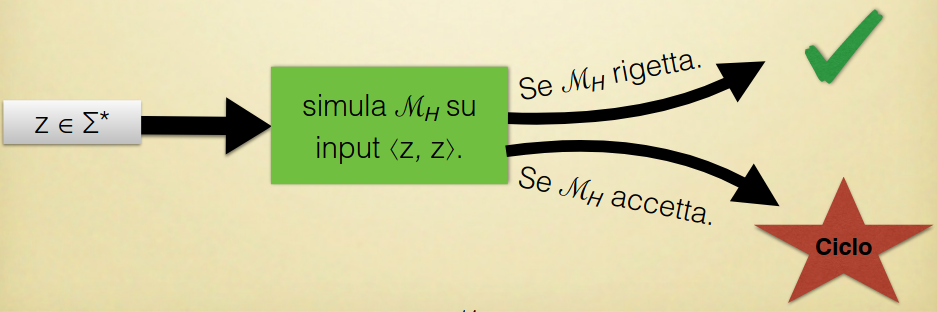
\includegraphics[scale=0.4]{TM_HALT2.png}\\
Proviamo ora ad  eseguire $M'$ su input $code(M')$.\\ 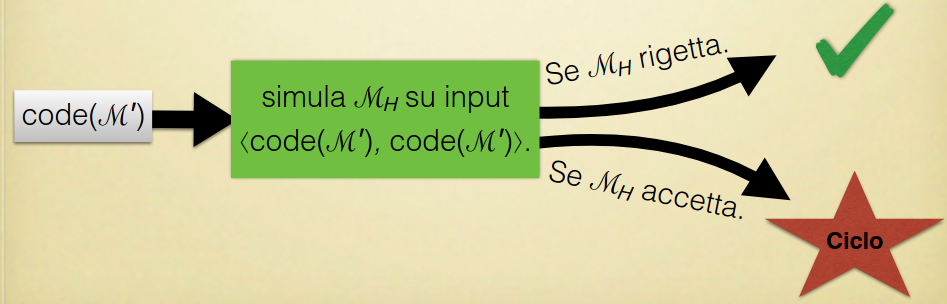
\includegraphics[scale=0.4]{TM_HALT3.png}
\\Dunque \\
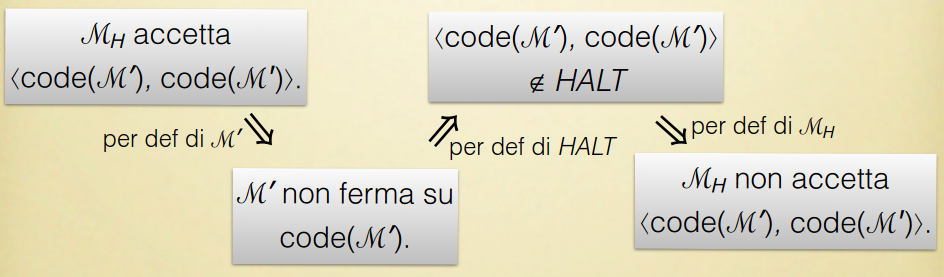
\includegraphics[scale=0.4]{HALT4.png}\\
Contraddizione. Proviamo il caso in cui rigetta.\\
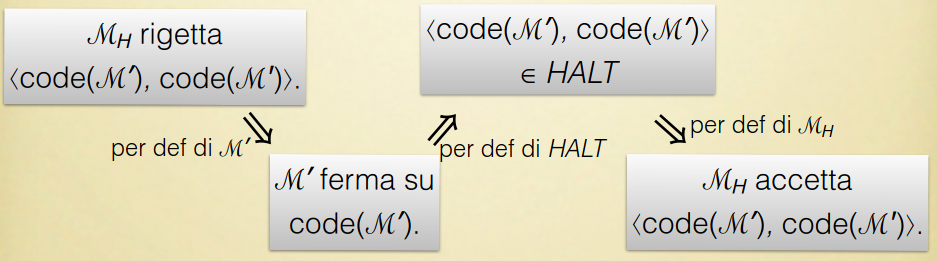
\includegraphics[scale=0.4]{HALT5.png}\\
Anche questo caso \`e in contraddizione. L'unica assunzione utilizzata nel costruire $M'$ \`e che $\exists M_H$ che decide HALT. Perci\`o $M_H$ non pu\`o esistere: HALT \`e indecidibile.
\end{enumerate}
\end{proof}

\subsection{Problemi non riconoscibili}
\begin{theorem}
Il complemento $HALT^{-}$ del problema della fermata non \`e riconoscibile da nessuna TM.
\begin{center}
$HALT$ = \{$\langle y,x \rangle \in \sum^{*}x\sum^{*}|$ y=code($M$) e $M$ ferma su x.\}
\end{center}
\begin{center}
$HALT^{-}$ = \{$\langle y,x \rangle \in \sum^{*}$x$\sum^{*}|$ y $\neq$ code($M$) $\forall$ $M$ o y=code($M$) e $M$ non ferma su x\}
\end{center}
\end{theorem}
C'\`e una dimostrazione diretta, per contaddizione, ma \`e pi\`u interessante mostrare una dimostrazione pi\`u astratta. Deriva dal seguente teorema.
\begin{theorem}
Se $HALT^{-}$ fosse riconoscibile, allora HALT sarebbe decidibile.
\end{theorem}
%Infatti, dal momento che HALT \`e indecidibile, se questo teorema \`e varo allora $HALT^{-}$ non pu\`o essere riconoscibile.
\begin{proof}
Abbiamo gi\`a visto che HALT \`e riconoscibile, diciamo da una TM $M_{HR}$. Supponiamo per assurdo che anche $HALT^{-}$ sia riconoscibile, e chiamiamo $M_{H^{-}}$ la TM che lo riconosce. Possimao ora costruire una TM $M_H$ che decide HALT come segue. Su input $\langle y,x \rangle$, simula $M_{HR}$ e $M_{H^{-}}$ in parallelo su input $\langle y,x \rangle$. Se $M_{HR}$ ferma, accetta. Se $M_{H^{-}}$ ferma, rigetta.\\
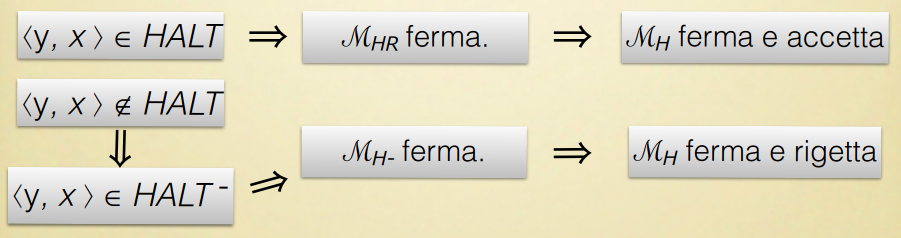
\includegraphics[scale=0.4]{TM_complemento_HALT.png}\\
Perci\`o $M_H$ decide HALT.
\end{proof}
Dal momento che HALT \`e indecidibile, allora $HALT^-$ non pu\`o essere riconoscibile.
\subsection{Osservazione 1. Complemento linguaggio riconoscibile}
La dimostrazione data non sfruttaa in alcun modo il fatto che HALT sia definito nel modo in cui \`e definito" potremmo sostituire HALT con qualsiasi problema riconoscibile, e funzionerebbe lo stesso. Abbiamo dunque il seguente teorema.
\begin{theorem}
\label{th:2}
Se $L$ e $L^{-}$ sono riconoscibili, allora $L$ \`e decidibile.
\end{theorem}
\begin{proof}
La stessa data per $L = HALT$
\end{proof}
Dai teoremi \ref{th:1} e \ref{th:2} otteniamo il seguente corollario.
\begin{corollary}
I linguaggi riconoscibili non sono chiusi sotto complemento.
\end{corollary}
\begin{proof}
HALT \`e riconoscibile ma il suo complemento non \`e riconoscibile.
\end{proof}
\subsection{Osservazione 2. Ridurre un problema ad un altro}
La nostra dimostrazione del fatto che $HALT^{-}$ non sia riconoscibile ha la seguente struttura:
\begin{center}
Se potessimo riconoscere L, allora potremmo decidere L'. Poich\`e non \`e decidibile, allora non possiamo riconoscere L.
\end{center}
Come ridurre L a L'? Vedremo come questa intuizione possa essere formalizzata in una tecnica di dimostrazione, che ci permette di ridurre problemi tra di loro al fine di dimostrarne la non calcolabilit\`a.
\section{esercitazione 1 Marzo 2023}
\subsection{Quesito 1}
Un problema che vogliamo risolvere usando uno strumento di calcolo puo' essere espresso come un problema di decisione. Questi problemi hanno la componente dei dati e la risposta SI/NO. Per poter risolvere questi problemi con un calcolatore e' necessario codificare un problema di decisinoe come la funzione caratteristica di un linguaggio formale.

Dato a e b dati le cui codifiche sono code(a) e code(b) $\in \sum^*$
Le proprieta' che la codifica deve rispettare sono: 
\begin{enumerate}
\item $a \ne b \ code(a) \neq code(b)$
\item deve essere verificabile che se x $\in \sum^*$ \`e $code(a)$ per qualche $a$
\item deve essere calcolabile a partire da $code(a).$
\end{enumerate}
\subsection{Problema 2.1}
Alfabeto $\sum = \{0,1\}$
La TM deve accettare l'input quando esso contiene 101 e rifiutare altrimenti.\\
\begin{tikzpicture}[shorten >=2pt,node distance=4cm,auto, on grid]

  \node[state,initial]   (1)  {$q_0$};
  \node[state, yshift=-1cm] (2) [right=of 1]  {$q_1$};
  \node[state, yshift=1cm] (3) [right=of 2]  {$q_2$};
  \node[state,accepting] (4) [right=of 3]  {$Y$};
  \node[state,accepting] (5) [below=of 2]	{$N$};

  \path[->]
  	(1) edge [loop above] node {$0,0,\rightarrow$} (1)
  	(1) edge [bend right] node {$\emptyset,\emptyset,\rightarrow$} (5)
	(1) edge  node {$1,1,\rightarrow$} (2)
	(2) edge [loop above] node {$1,1,\rightarrow$} ()  	
  	(2) edge  node {$\emptyset,\emptyset,\rightarrow$} (5)
  	(2) edge  node {$0,0,\rightarrow$} (3)
  	(3) edge [] node {$1,1,\rightarrow$} (4)
  	(3) edge [bend right, above] node {$0,0,\rightarrow$} (1)
  	(3) edge [bend left] node {$\emptyset,\emptyset,\rightarrow$} (5)
  	;
  	
\end{tikzpicture}

\subsection{Problema 2.2}
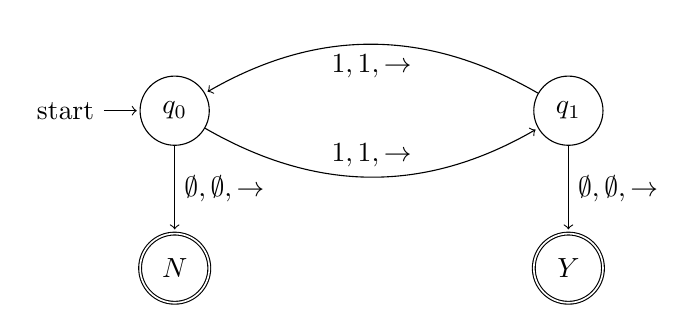
\begin{tikzpicture}[shorten >=1pt,node distance=5cm,auto, on grid]
	\node [state, initial] (1) {$q_0$};
	\node [state] (2) [right=of 1] {$q_1$};
	\node [state, accepting, yshift=3cm] (3) [below=of 1] {$N$};
	\node [state, accepting, yshift=3cm] (4) [below=of 2] {$Y$};
	
	\path[->]
		(1) edge [bend right] node  {$1,1,\rightarrow$} (2)
		(2)	edge [bend right] node  {$1,1,\rightarrow$} (1)
		(1) edge node  {$\emptyset,\emptyset,\rightarrow$} (3)
		(2) edge node  {$\emptyset,\emptyset,\rightarrow$} (4)
		;

\end{tikzpicture}



\section{Linguaggi sono non numerabili}
Sia $S_{\sum}$ l'insieme di tutti i linguaggi sull'alfabeto finito $\sum$.
\begin{theorem}
L;insieme $S_{\sum}$ non \`e numerabile.
\end{theorem}
\begin{proof}
Ricorda che un linguaggio L \`e un sottoinsieme di $\sum^*$. Abbiamo gi\`a visto che $\sum^*$ \`e infinito numerabile, quindi possiamo scriverlo come $\sum^* = \{\sigma_1, \sigma_2,\sigma_3,...\}$. Allora un linguaggio, diciamo $L_1 = \{\sigma_1,\sigma_4\}$, pu\`o essere rappresentato come una riga in una tabella:\\
\begin{center}
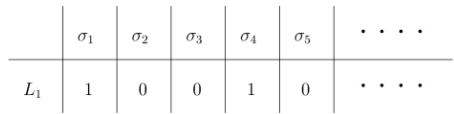
\includegraphics[scale=0.5]{tabella_linguaggi.png}

\end{center}
\end{proof}
Ciascun linguaggio su $\sum$ pu\`o essere rappresentato in questo modo. Per contaddizione, assumi che $S_{\sum}$ sia un insieme numerabile. Allora possiamo assegnare un numero naturale ai suoi elementi, cos\`i che ogni $L_i \in S_{\sum}$ appare come riga a destra.\\ \begin{center}
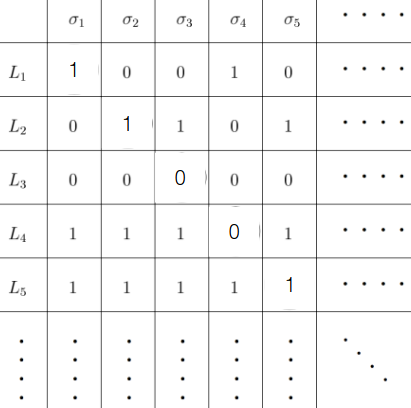
\includegraphics[scale=0.5]{tabella_linguaggi2.png}
\end{center}
Davvero ogni elemento $L$ di $S_{\sum}$ compare su una riga?\\
Definisci $L$ come $00110...$, allora $\sigma_i \in L \iff \sigma_i \notin L_i$. Quindi $L$ \`e diverso da ogni linguaggio $L_i$ sulla riga. Dunque $L$ non pu\`o essere in una riga! \textbf{Contraddizione}.\\ Quindi, $S_{\sum}$ non \`e numerabile.\\ \begin{center}
 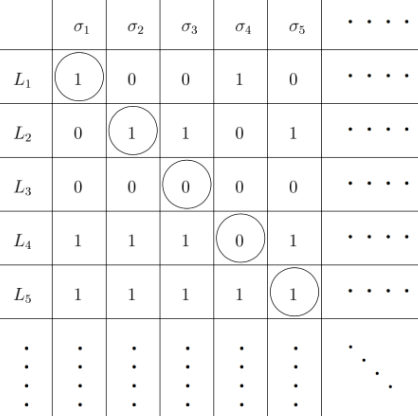
\includegraphics[scale=0.5]{tabella_linguaggi3.png}
\end{center}
\subsection{Riassumendo}
Dato un alfabeto finito $\sum$, abbiamo visto che:
\begin{enumerate}
\item l'insieme di linguaggi riconoscibili da una TM \`e infinito numerabile.
\item l'insieme di tutti i linguaggi \`e non-numerabile.
\end{enumerate}
Quindi, esistono limguaggi che non sono riconoscibili da alcuna TM, ad esempio $HALT^{-}, EQ, EQ^{-}$.\\
\subsubsection{Quanti linguaggi non riconoscibili ci sono?}
La risposta deriva da un  un risultato generale.
\begin{theorem}
\label{th:3}
Se $S$ \`e un insieme infinito, non-numerabile e $S'$ \`e un sottoinsieme infinito numerabile di S, allora $S \backslash S'$ non \`e un inifinito numerabile.
\end{theorem}
\begin{proof}
Assumi $S \backslash S'$ sia infinito numerabile. Allora, poich\`e i linguaggi infiniti numerabili sono chiusi per unione, $(S \backslash S') \cup S' = S$ \`e numerabile. Contraddizione!
\end{proof}
Dal \ref{th:3} otteniamo il seguente corollario.
\begin{corollary}
L'insieme di linguaggi non riconoscibili non \`e infinito numerabile, allora ci sono pi\`u linguaggi non riconoscibili che riconoscibili.
\end{corollary}


\section{Teorema di Rice}
Abbiamo visto che non possiamo decidere se una TM: \begin{enumerate}
\item ferma su un dato input
\item ferma su input vuoto (stringa vuota)
\item \`e equivalente a un\`altra TM.
\end{enumerate}
Allora, quali problemi riguardanti le TM sono decidibili?
Per esempio: \begin{enumerate}
\item possimo verificare quanti stati ha una macchina, e desumere quanti stati ha
\item se va mai a dx o a sx
\end{enumerate}
Cos'altro?
\subsection{ripasso: linguaggi}
Una \textbf{propriet\`a di linguaggio} P \`e una funzione da un insieme di TM a ${0,1}$ (falso/vero), tale che $L_M = L_{M'}$ implica P($M$) = P($M'$).
Questo assicura che P dipenda solo dal linguaggio descritto dalla macchina. Per esempio: "ferma in 42 step" non \`e propriet\`a del linguaggio.
Questa propriet\`a \`e \textbf{non-triviale} se esiste una TM $M$ tale che P($M$) - 1 e una TM $M'$ tale che P($M'$)=0. Formalmente, identificheremo le TM che soddisfano la propriet\`a P con l\`insieme: \begin{center}
$\{y \in \sum^* | y=code(M)\ e\ P(M)=1\}$
\end{center} 
\subsection{Teorema di Rice}
\begin{theorem}
Se P \`e una propriet\`a di lunguaggio non triviale, allora il problema "M ha propriet\`a P" \`e indecidibile.
\end{theorem}
\begin{proof}
Per contraddizione  dimostraiamo che se "$M$ ha propriet\`a P" fosse decidibile, allora il problema della fermata sarebbe decidibile.\\
Considera una prpriet\`a P. Assumiamo P($M_{\emptyset}$) = 0. ($M_{\emptyset}$ \`e una TM che riconosce il linuaggio vuoto.) Poich\`e P \`e non-triviale, possiamo considerare una TM $M_P$ tale che P($M_P$) = 1. Fissiamo $M$ e x come parametri e costruiamo la seguente TM $M_{M,x}$:\\
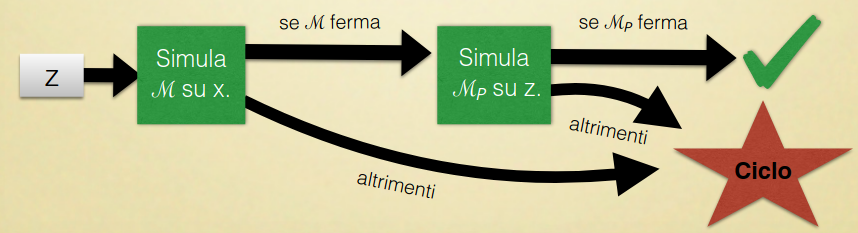
\includegraphics[scale=0.5]{TM_RICE1.png}\\
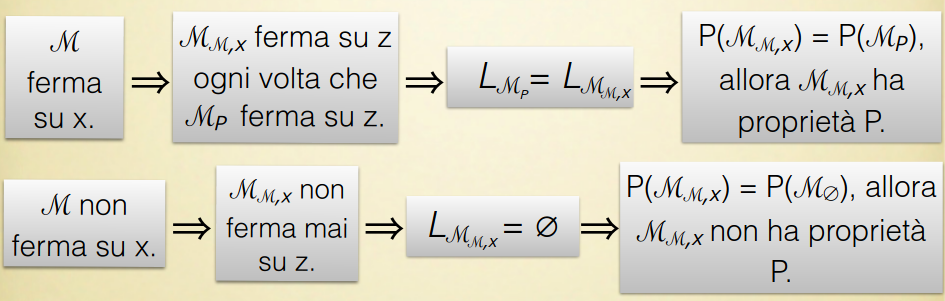
\includegraphics[scale=0.45]{RICE2.png}\\
Se potessimo decidere se $M_{M,x}$ ha la propriet\`a P, potremmo decidere il problema della fermata. Allora, $\{y|y=code(M) e P(M)=1\}$ \`e indecidibile.\\
Abbiamo assunto P($M_{\emptyset}$)=0. Se P($M_{\emptyset}$)=1? In questo caso, ripetiamo lo stesso argomento, ma per la propriet\`a $\neg P$ ("$M$ non ha la propriet\`a P"). Osserva che questo funziona perch\`e: \begin{enumerate}
\item dato che P \`e non-triviale, anche $\neg P$ \`e non-triviale.
\item dato che P($M_{\emptyset}$) = 1, allora $\neg P(M_{\emptyset}) = 1\}$ \`e indecidibile.
\end{enumerate}
Concludiamo che $\{y|y=code(M) \land \neg P(M) = 1\}$ \`e indecidibile. Questo implica che anche $\{y | y=code(M) \land P(M)=1\}$ sia indecidibile.
\end{proof}
NB: lo schema di dimostrazione \`e:
\begin{itemize}
\item Devo dimostrare $A \iff B$
\item Dimostriamo $A \Rightarrow B \land \neg A \Rightarrow \neg B$
\item Che equivale a $A \Rightarrow B \land B \Rightarrow A$
\end{itemize}
\end{document}



























